

\documentclass{article}
\usepackage[utf8]{inputenc}
\usepackage{authblk}
\usepackage{setspace}
\usepackage[margin=1.25in]{geometry}
\usepackage{graphicx}
\graphicspath{ {./figures/} }
\usepackage{subcaption}
\usepackage{amsmath}
\usepackage{lineno}
\usepackage{booktabs}% pour les table depuis R
\usepackage{makecell}
\linenumbers

%%%%%% Bibliography %%%%%%

\usepackage[
    style=nejm, 
    citestyle=numeric-comp,
    sorting=none, 
    backend=biber]{biblatex}

\addbibresource{treeModel.bib}

%%%%%% Title %%%%%%
% Full titles can be a maximum of 100 characters, including spaces. 
% Title Format: Use title case, capitalizing the first letter of each word, except for certain small words, such as articles and short prepositions
\title{From Local Actors to Leaf Protectors: A Collaborative Modeling Approach for Rethinking Tree Management and Protection Measures in Senegal's Groundnut Basin}

%%%%%% Authors %%%%%%
% Authors should be listed in order of contribution to the paper, by first name, then middle initial (if any), followed by last name.
% Authors should be listed in the order in which they will appear in the published version if the manuscript is accepted. 
% Use an asterisk (*) to identify the corresponding author, and be sure to include that person’s e-mail address. Use symbols (in this order: †, ‡, §, ||, ¶, #, ††, ‡‡, etc.) for author notes, such as present addresses, “These authors contributed equally to this work” notations, and similar information.
% You can include group authors, but please include a list of the actual authors (the group members) in the Supplementary Materials.
\author[1,2,6*$\dag$]{E. Delay}
\author[1,2,4$\dag$]{L. Broutin}
\author[1,2]{A. Fallot}
\author[3]{A. Perrotton}
\author[4]{A. Gonin}
\author[5]{D. Masse}


%%%%%% Affiliations %%%%%%
\affil[1]{CIRAD, UMR SENS, F-34398 Montpellier, France.}
\affil[2]{SENS, CIRAD, IRD, Université de Paul Valéry Montpellier 3, Montpellier, France.}
\affil[3]{Forêts et Sociétés, Univ Montpellier, CIRAD, Montpellier, France.}
\affil[4]{Université Paris Nanterre, Laboratoire LAVUE, FR.}
\affil[5]{IRD, Eco\&Sols, Abidjan, Côte d’Ivoire.}
\affil[6]{UMI UMMSCO,  Université Cheick Anta Diop, Dakar, Sénégal.}
\affil[*]{Address correspondence to: etienne.delay@cirad.fr}
\affil[$\dag$]{These authors contributed equally to this work.}

%%%%%% Date %%%%%%
% Date is optional
\date{}

%%%%%% Spacing %%%%%%
% Use paragraph spacing of 1.5 or 2 (for double spacing, use command \doublespacing)
\onehalfspacing

\begin{document}

\maketitle

%%%%%% Abstract %%%%%%
\begin{abstract}

    How can a participatory simulation model contribute to understanding the socio-ecological dynamics and fostering innovative strategies for sustainable management of trees, crops, and pastoralism in the peanut basin?

    In the agro-pastoral zones, the Sahelian ecosystems have undergone significant degradation, characterized by a reduction in tree cover, as a consequence of the droughts in the 1960s and 1990s. The peanut basin stands out for its positive interrelationships between trees, crops, and pastoralism. However, the regeneration of the Faidherbia park has declined since the major droughts. Through collaborative efforts with agro-pastoral farmers, we have developed a simulation model -- The SAFIRe model : Simulation of Agents for Fertility, Integrated Energy, Food security, and Reforestation-- that aims to unravel the complex social and ecological dynamics at play and explore potential strategies in partnership with local communities.

    By exploring the results of the model co-designed with local stakeholders, we have identified more effective management strategies, as per the request of the local actors. However, more importantly, we have collectively questioned the conditions for improving tree cover and the viability of the socio-ecosystem, particularly in relation to the demand for firewood and local cereal for sustenance. This has prompted the stakeholders to engage in community-wide discussions and transform agro-pastoralists into leaf protectors.

\end{abstract}

%%%%%% Main Text %%%%%%

\section{Introduction}
%Your manuscript should contain all of the numbered sections specified in this template: Introduction, Results, Discussion, Materials and Methods.

%The manuscript should start with a brief introduction that lays out the problem addressed by the research and describes the paper’s importance. The scientific question being investigated should be described in detail. The introduction should provide sufficient background information to make the article understandable to readers in other disciplines and provide enough context to ensure that the implications of the experimental findings are clear. 

Il est treize heures, la brousse d’avril est vide et silencieuse. Aucun animal en vue, aucun Homme à l’horizon, presque aucun signe de vie. Difficile d’imaginer que ces espaces sableux verront se précipiter laboureurs et planteurs d’ici peu. Les arbres eux sont là, seules petites touches vertes dans ce paysage séché. Leur ombrage est précieux mais il faut affronter le soleil pendant de longues minutes pour s’y réfugier. Ils demeurent loin les uns des autres, de façon étonnamment régulière. Plus saisissant encore : leur taille. Ce n’est pas qu’ils soient bien grands, mais tous semblables. Ils ont surement tous le même âge ! Et si c’est le cas, ils finiront tous par mourir en même temps.

La région sahélienne a été le témoin d'une série de sécheresses dévastatrices s'étalant des années 1960 aux années 1990, ayant provoqué une dégradation substantielle de ses écosystèmes, en particulier par la réduction significative de leur couvert arboré \cite{mbow_what_2015}. Cette perte de couvert arboré a eu des conséquences néfastes, se traduisant par une diminution des services écosystémiques essentiels fournis à la population et à la biodiversité. Cependant, l'ampleur de cette perte de SE est d'autant plus préoccupante que la population de la région sahélienne ne cesse de croître rapidement \cite{cesaro_reforestation_2023}. Dans un contexte de pénurie, l'utilisation intensive des ressources naturelles par l'agriculture et l'élevage aggrave la dégradation des terres et de la fertilité des sols \cite{tappan_landscapes_2016}.

En 2018, un constat alarmant mettait en lumière le fait que près de 40\% de la population mondiale était exposée aux conséquences de la dégradation des sols (Monique Barbut, Secrétaire exécutive de la Convention des Nations Unies sur la lutte contre la désertification). Dans ce contexte, les enjeux liés à la conservation et à la restauration de la fertilité des sols demeurent cruciaux. 
C'est dans ce contexte qu'a émergé l'initiative "4 pour 1000" (4p1000) en 2015, une proposition visant à accroître la séquestration du carbone dans les sols agricoles, présentée comme une solution pour améliorer la fertilité des sols et contribuer à l'atténuation du changement climatique \cite{kon_kam_king_soil_2018}.

Ester Boserup (1965) a avancé l'idée que la baisse de la fertilité des sols pousse les agriculteurs à intensifier leurs pratiques. Les travaux antérieurs cherchant à établir des liens entre phénomènes sociaux et pratiques agricoles se sont souvent centrés sur l'intensification. Toutefois, dans le cadre du projet de recherche et développement DSCATT (Dynamique de la Séquestration du Carbone dans les sols des systèmes agricoles Tropicaux et Tempérés), qui s'inscrit dans l'initiative 4p1000, notre objectif était de comprendre les relations qu'entretiennent les populations locales du bassin arachidier sénégalais avec les arbres. Pour ce faire, nous avons examiné les usages des arbres et les pratiques de gestion des populations locales afin de construire un modèle de simulation co-construit: le modèle SAFIRe (Simulation of Agents for Fertility, Integrated Energy, Food security, and Reforestation). Cette approche s'inscrit dans un cadre de Modélisation d'accompagnement (ComMod) \cite{etienne_companion_2014,barreteau_our_2003} et d'Exploration d'accompagnement (ComExp) \cite{delay_comexp_2020} visant à explorer collectivement les futurs possibles pour le territoire.

Dans le contexte de la gestion durable des terres, les options de restauration identifiées par les paysans sont étroitement liées à la surveillance des arbres pour réduire les risques de prédation par les populations avoisinantes. Deux pistes d'exploration ont émergé des échanges avec les communautés locales : l'influence de la surveillance déléguée aux agents des eaux et forêt, ainsi que les conditions de développement du parc arboré lorsque la surveillance reste sous la responsabilité de la population. Cette étude vise à approfondir ces aspects dans le but de contribuer à une meilleure compréhension des pratiques de gestion durable des ressources naturelles et de la biodiversité dans un contexte sahélien en mutation.

% %%%%% Citations in the text %%%%%%
% \subsection*{Citations}
% Citations of references in the text should be identified using numbers in square brackets e.g., ``as discussed by Cui \cite{Cui1}'' or ``as discussed elsewhere \cite{Cui1,Ninomiya1,Li1,Wang1,Yang1}.'' All references should be cited within the text and uncited references will be removed. 

% As an example, this template includes a ``sample.bib'' file containing the references in BibTeX.

% %%%%%% Equations %%%%%%
% \subsection*{Equations}
% Equations should be provided in a text format, rather than as an image. Equations should be numbered consecutively, in round brackets, on the right-hand side of the page by using the ``\textbackslash begin\{equation\}'' command. They should be referred to as Equation 1, etc. in the main text.

% \medskip For example, see Equation \ref{eq:1} and Equation \ref{eq:2} below.
% \begin{equation} \label{eq:1}
%     a^2 + b^2 = c^2
% \end{equation}
% \begin{equation} \label{eq:2}
% \begin{split}
% A & = \frac{\pi r^2}{2} \\
%  & = \frac{1}{2} \pi r^2
% \end{split}
% \end{equation}

% %%%%%% Figures %%%%%%
% \subsection*{Figures}
% Figures should be called out within the text and numbered in the order of their citation in the text. Every figure must have a descriptive title beginning with ``Figure [Number] …'' All figure titles should be either a phrase or a sentence; do not mix the two styles. See Figure \ref{fig:1} for example.
% \begin{figure}[h]
%     \centering
%     
\includegraphics[width=0.5\textwidth]{./img/fig 1}
%     \caption{This is an example figure.}
%     \label{fig:1}
% \end{figure}

% Figures should be displayed on a white background. When preparing figures, consider that they can occupy either a single column (half page width) or two columns (full page width), and should be sized accordingly.

% If a figure consists of multiple panels, they should be ordered logically and labelled with roman letters (i.e., A, B, C, etc.). All labels should be explained in the legend. See Figure \ref{fig:2} for example.

% Upon acceptance, authors will be asked to provide the figures as separate electronic files. At that stage, figures should be supplied as Adobe Portable Document Format (PDF), PostScript (PS), or Encapsulated PostScript (EPS) for illustrations or diagrams; Tagged Image File Format (TIFF), JPEG, PNG, PhotoShop (PSD), EPS, or PDF for photography or microscopy. Bitmap (BMP) images should be of at least 300 dpi resolution, unless due to the limited resolution of a scientific instrument. If a bitmap image has labels, the image and labels should be embedded in separate layers.

% \begin{figure}[h]
%     \centering
%     \begin{subfigure}{0.4\textwidth}
%         
\includegraphics[width=0.9\textwidth, height=2in]{./img/fig 1}
%         \caption{\label{fig:2a}}
%     \end{subfigure}
%     \begin{subfigure}{0.4\textwidth}
%         
\includegraphics[width=0.9\textwidth, height=2in]{./img/fig 2}
%         \caption{\label{fig:2b}}
%     \end{subfigure}
%     \caption{This is an example of a figure consisting of multiple panels.     (\subref{fig:2a}) This is the first panel. (\subref{fig:2b}) This is the second panel.}
%     \label{fig:2}
% \end{figure}

% %%%%%% Tables %%%%%%
% \subsection*{Tables}
% Tables should supplement, not duplicate, the text. They should be called out consecutively within the text and numbered in the order of their citation in the text. 

% Every table must have a descriptive title beginning with ``Table [Number] …'' as noted in Table \ref{tab:1}. If numerical measurements are given, the units should be included in the column heading. Every vertical column should have a heading, followed by a unit of measure (if any) in parentheses. Units should not change within a column. Vertical rules should not be used. 

% Centered headings of the body of the table can be used to break the entries into groups. Do not use footnotes in column heads; include any such details in sentence form in the table legend. Footnotes should contain information relevant to specific cells of the table; use lowercase letters in alphabetical order, as needed: a, b, c, etc. 

% \begin{table}[b]
%     \caption{This is an example table.}    
%     \centering
%     \begin{tabular}{ccc}
%             \hline
%             Column 1 & Column 2 & Column 3 \\  
%             \hline
%             Cell 1 & Cell 2 & Cell 3\\ 
%             Cell 4 & Cell 5 & Cell 6 \\
%             \hline
%             \end{tabular}

%     \label{tab:1}
% \end{table}

\section{Materials and Methods}

Le Sommet de Rio en 1992 a marqué un tournant majeur dans la manière dont la gestion des ressources naturelles est perçue. Il a contribué à la démocratisation de la notion de gestion basée sur les communautés, favorisant le passage d'une vision autoritaire de la gestion des ressources à des approches plus intégrées \cite{delay_coming_2022}. Cette évolution a reconnu l'importance d'impliquer activement les parties prenantes locales dans la prise de décision et la gestion de leurs environnements naturels. Cependant, cette intégration des communautés dans les processus de gestion des ressources a engendré des défis complexes, notamment en ce qui concerne la co-construction de représentations et de compréhensions communes de ces environnements.

L'intégration des acteurs hétérogènes au sein de collectifs pour co-construire des modèles et des simulations s'est révélée être une réponse novatrice à ces défis. Complètement compatible avec la philosophie de la modélisation d'accompagnement, cette approche a donné naissance à des méthodes novatrices. Dans le cadre de nos travaux, nous avons animé des ateliers visant à élaborer une méthode d'anticipation que nous avons nommée ACARDI \cite{perrotton_definition_2021}. Cette méthode repose sur la collaboration étroite entre chercheurs et acteurs locaux, mettant en avant la co-construction de modèles et de simulations pour anticiper les évolutions des territoires. A l'issu du processus, nous étions face au premier Living-Lab de l'observatoire de Niakhar.

Après avoir mené des ateliers participatifs à Diohine, impliquant activement les acteurs locaux, nous avons identifié un certain nombre d'aspirations et de préoccupations spécifiques des populations pour leur territoire. Parmi celles-ci, l'aspiration au "retour de la faune et de la flore" a retenu notre attention particulière. Pour explorer cette aspiration de manière plus approfondie, nous avons associé une démarche anthropologique à la co-construction d'un modèle de simulation. Cette section se penche sur notre approche et notre méthodologie visant à donner vie à cette aspiration, en combinant les aspects socio-culturels et les outils de modélisation pour une compréhension holistique.

\subsection{Modelling for Empowerment - An Anthropological Approach to Participatory Model Co-construction}

La mise en œuvre des ateliers ACARDI a ouvert la voie à une phase cruciale de notre recherche, marquée par une immersion de trois mois à Diohine. Cette immersion a été conçue pour aller au-delà des discussions en atelier et a permis d'entreprendre un travail de collecte d'informations approfondi en utilisant des entretiens et l'observation participante. Cet investissement sur le terrain a été essentiel pour comprendre de manière plus nuancée les aspirations et les préoccupations des populations locales en matière de gestion de leurs territoires.

Au fil de ces entretiens et de l'observation participante, un processus de développement de modèles conceptuels a été enclenché, évoluant progressivement vers la création d'un modèle informatique basé sur des agents. La co-construction de ces modèles a été une démarche collaborative et itérative, impliquant activement le groupe d'acteurs du Living-Lab de Diohine. Les acteurs locaux ont joué un rôle clé en discutant, en évaluant et en validant chaque aspect de ce modèle, contribuant ainsi à son ajustement pour refléter au mieux leurs réalités et leurs attentes.

Après une validation approfondie du modèle avec les acteurs locaux, dans une démarche qualifiée de validation à dire d'expert \cite{bommel_definition_2009}, nous avons entamé un travail d'exploration du modèle à l'aide de la plateforme OpenMole \cite{reuillon_openmole_2013}. Cette phase d'exploration nous a permis de simuler divers scénarios et de recueillir des résultats significatifs, qui nécessitaient ensuite d'être présentés aux participants du Living-Lab pour recueillir leurs avis et approfondir la discussion. Pour faciliter cette étape cruciale, nous avons développé une interface interactive, conçue pour simplifier la manipulation et la validation de grandes quantités de données par les acteurs, tout en assurant une expérience fluide et collaborative.

\begin{quote}
"mais en quoi l’expérience du voyage anthropologique propose t-elle de renouveler ou de reconsidérer l’épistémologie du déplacement (de l’un vers l’autre) ? Par-delà la constitution des objets des sciences sociales, ethnies, cultures, sociétés, en quoi le voyage du sujet est-il progressivement devenu vecteur de la réflexion théorique ? "
\end{quote}

\subsection{ODD }

    Dans cette section nous allons décrire le modèle The SAFIRe model (Simulation of Agents for Fertility, Integrated Energy, Food security, and Reforestation) en utilisant le framwork de description ODD \cite{grimm_standard_2006,grimm_odd_2010,grimm_odd_2020}.

    \subsubsection{Overview}

        \textbf{Purpose}

        The peanut basin is facing a loss of soil fertility. Chemical amendments are either unavailable in the area or economically inaccessible for farmers. Therefore, soil fertility depends on two aspects: the presence of livestock in the territory to maintain year-round manure, and the Faedherbia albida trees which play a fundamental role in crop cycles. Indeed, these trees have the unique characteristic of shedding their leaves during the growing season and fixing nitrogen from the air into the soil.

        The model thus aims to evaluate and explore solutions for managing the Faedherbia park to increase their density. The model focuses on exploring so-called community initiatives.

        The objective of this study was co-defined with the participants based on their desire to restore trees and biodiversity. According to their perspective, the decline in tree population is strongly linked to individual practices associated with pastoralism. Thus, the aim was to reassess the functioning of their system, the role of "tree cutters," and the optimization of surveillance by comparing community-based surveillance efforts with centralized surveillance conducted by them and the forestry department.\\

        Throughout the study, we also examined the role of farmers and agro-pastoralists in the disappearance of trees. It was observed that young tree seedlings are no longer marked and destroyed by animal-drawn tools.

        \textbf{Entities, state variables and scales}

        The entities in the model are relatively numerous: some are static (trees, plots, and village), while others are in motion (shepherds, farmers, woodcutters, and overseers). 

        patches : nbarbresici: Number of trees present on this patch; arbre-ici: Indicates if there is a tree on this patch (reference to a specific tree); tree-influence: Influence of the tree on this patch (can represent aspects like shade, nutrients affected by the tree, etc.); under-tree: (TRUE/FALSE) Indicates if the patch is under a tree; culture: Type of crop on this patch (can be millet or groundnut); en-culture: Indicates if the patch is currently used for crops; rendement-mil-g: Yield of millet on the patch in terms of grains (to be calibrated later); rendement-mil-p: Yield of millet on the patch in terms of bundles; rendement-groundnuts-g: Yield of groundnuts on the patch in terms of grains; rendement-groundnuts-p: Yield of groundnuts on the patch in terms of bundles; id-parcelle: Identifies the parcel, allowing the structure of the parcels to be maintained during rotation; pas-rotation: Tracks parcels that have not yet rotated (system of +1); rotation: (TRUE/FALSE) Indicates if the parcel has already undergone rotation; champ-brousse: Indicates if the patch is in bushland; zoné: (TRUE/FALSE) Indicates if the patch is used for defining fallow zones; zone: Indicates to which fallow rotation zone the patch belongs (there are 3 zones for fallow rotation).

        Trees : proche-village: Likely unnecessary variable (trees in villages are also pruned); nb-coupes: Number of cuts; nb-jour-coupe: Number of cutting days; age-tree: Age of the tree. Trees have olso a subclass Saplings composed by age: Age in days ; signalé: Reported; rna-coupe: Cut in RNA.


        farmers : id-agri: Links to the farmer's unique parcel; engagé: TRUE/FALSE engagement in the Assisted natural regeneration (RNA in fr); interet-RNA: Interest in the RNA; jour-champ: Days spent in the field; nb-ha-a: Number of hectares allocated; stock-mil: Stock of millet; idMyBerger: Identifier of the associated shepherd; nb-patches: Number of patches; mon-chp-RNA: Field in the RNA.


        hearder : troupeau-nourri: does the herd have enough to eat, currently TRUE/FALSE; arbre-choisi: tree chosen to be cut and fed to animals as fodder ; nb-têtes: herd size for the shepherd ; nb-ha-b: Between 3.8 (newly settled, 11\%) and ~5.5 (89\% of the population); stock-fourrage: Forage stock; idAgri: Identifier of my reference farmer.

        woodcutters : attrape: Captured (TRUE/FALSE); nb-attrape: Number time he was captured; jours-peur: Days of fear after capuration; en-coupe: Currently cutting.


        The simulated space, through which the agents interact, represents 100 hectares. It is composed of 1000 spatial entities (patches) with a size of 10 square meters (resolution). It is exclusively agricultural since the inhabited area of the village is condensed into a single point. (The areas that are not cultivated, such as wetlands and pathways, are rare and have not been represented.)

        The irreducible time step is one day (tick). The various elements of the system (interactions, etc.) take into account the seasonality that structures agricultural activities. Every 364 days, a new year begins and the rhythm of the seasons continues. A second time unit can be considered: the year, which consists of seasons. Simulations are generally carried out over 23 years. At the beginning of the simulation, the first 3 years are considered to initialize the model.

    
        \textbf{Process overview and scheduling}\\

        This section provides an overview of the processes and their scheduling within the model. The model is composed of several sub-models that simulate various aspects of the ecosystem and human activities. Each process is organized and executed in a specific sequence to reflect the interactions and dependencies within the system. The following describes repeated procedures that occur at each time step:

        \begin{itemize}
            \item Harvest and Crop Management
            \begin{itemize}
                \item Harvest and stockpiling: Farmers harvest crops and store them in their stockpiles.
                \item Effect of machinery on unprotected saplings: Machinery used in the fields may damage or destroy unprotected saplings.
                \item Crop rotation: Farmers rotate crops between different fields to maintain soil fertility and reduce pest buildup.
            \end{itemize}

            \item Tree Growth and Reproduction
            \begin{itemize}
                \item Sprouting: New saplings sprout around mature trees, influenced by tree density and environmental conditions.
                \item Sapling growth: Saplings grow over time, with growth rates dependent on available resources and environmental factors.
                \item Aging and death of trees: Trees age and may eventually die due to old age, disease, or other environmental factors.
            \end{itemize}

            \item Livestock Feeding and Forage Use of Acacias
            \begin{itemize}
                \item Feeding livestock with straw: Shepherds feed their livestock with straw collected from the fields.
                \item Tree cutting: Trees are cut down for forage or other uses by the shepherds.
                \item Livestock in fallow land and cutting of saplings: Livestock graze in fallow lands, and shepherds may cut down saplings to manage the land.
            \end{itemize}

            \item Cutting of Saplings by Woodcutters
            \begin{itemize}
                \item Detection of saplings: Woodcutters search for and identify saplings that can be cut.
                \item Cutting of saplings: Once identified, saplings are cut by the woodcutters for use as firewood or other purposes.
            \end{itemize}

            \item Farmer Engagement
            \begin{itemize}
                \item Participation in meetings: Farmers participate in community meetings to discuss agricultural practices and share knowledge.
                \item Observing the success of neighbors: Farmers observe the practices and successes of their neighbors to learn and adapt.
                \item Social interaction and motivation: Social interactions among farmers influence their motivation and engagement in community activities.
                \item Protection of saplings: Farmers take actions to protect saplings from damage by livestock or machinery.
            \end{itemize}

            \item Surveillance
            \begin{itemize}
                \item Surveillance and presence of farmers in the fields (generalized community surveillance): Farmers patrol their fields and monitor for any issues such as pests or unauthorized grazing.
                \item Delegated community surveillance: Specific individuals or groups are assigned the task of community surveillance to ensure all fields are monitored effectively.
            \end{itemize}
        \end{itemize}


    \subsubsection{Design Concepts}
        \textbf{Basic principles}\\

        

        \textbf{Objectives}\\
        \textbf{Adaptation}\\
        
        Two agents exhibit adaptive/changing behaviors: the woodcutters and the farmers. The response of the woodcutters to being caught by a sapling protector varies according to the number of times they have been caught previously. Farmers have a score describing their interest in tree protection. This score evolves constantly according to several rules: encountering another engaged farmer, observing the success of a neighbor's protection system, participating in meetings, etc.

        \textbf{Emergence}\\
        \textbf{Sensing}\\
        \textbf{Interaction}\\

        The interaction between agents is direct. Woodcutters interact directly with the saplings by cutting them down. Similarly, shepherds interact directly with the trees by utilizing them for forage. Farmers and supervisors also have direct interactions with woodcutters by stopping them from cutting the saplings. Additionally, farmers destroy young saplings that are not protected.

        \begin{itemize}
            \item \textbf{Woodcutters and Saplings}: Woodcutters seek out saplings and cut them down for use as firewood or other purposes. This direct interaction reduces the number of saplings in the environment.
            \item \textbf{Shepherds and Trees}: Shepherds interact with trees by feeding their livestock with tree foliage or cutting down trees for forage. This direct interaction affects the tree population and influences the availability of forage resources.
            \item \textbf{Farmers and Woodcutters}: Farmers interact with woodcutters by attempting to stop them from cutting saplings. When farmers encounter woodcutters in the field, they may intervene to protect the saplings.
            \item \textbf{Supervisors and Woodcutters}: Supervisors, acting as protectors, also interact directly with woodcutters. They monitor the fields and stop woodcutters from cutting down saplings to ensure the protection of young trees.
            \item \textbf{Farmers and Unprotected Saplings}: Farmers destroy young saplings that are not protected. This interaction occurs when farmers are working in their fields and come across unprotected saplings, which they remove to prevent interference with their crops.
        \end{itemize}

        \textbf{Stochasticity}\\

        Many events in the model rely on stochasticity since they are probabilistic. Probability is often used as a frequency measure. This is the case for the movements of farmers in their fields and the probability that farmers will discuss the RNA (Assisted natural regeneration) with each other.

        Stochasticity is used to represent uncertainty, particularly concerning whether supervisors catch woodcutters. Since supervisors do not spend the entire day in a single field, they may visit a field without encountering the woodcutter.

        Finally, randomness is used to create variability in initial conditions. This is the case for the number of heads in different herds, which vary in size, and for the initial age of each tree, resulting in trees of varying ages.

        \begin{itemize}
            \item Partial Randomness as Uncertainty
            \begin{itemize}
                \item Farmer Movements: The movements of farmers within their fields are determined randomly. This means that their location at any given time is based on a probability distribution, ensuring variability in their positions.
                \item Discussions about RNA: The likelihood that farmers will engage in discussions about the RNA is also probabilistic. This frequency-based probability allows for random interactions among farmers, influencing their engagement with the RNA.
                \item Supervisors and Woodcutters: The uncertainty in supervisors catching woodcutters is modeled using partial randomness. Supervisors patrol fields but may not always encounter woodcutters due to the random nature of their patrol routes and the woodcutters' activities.
            \end{itemize}

            \item Randomness for Initial Variability
            \begin{itemize}
                \item Herd Sizes: The initial number of heads in each herd is determined randomly, resulting in herds of varying sizes. This introduces variability into the model, reflecting real-world differences in herd sizes.
                \item Tree Ages: The initial age of each tree is assigned randomly, creating a population of trees with a range of ages. This variability in tree ages ensures a more realistic representation of a forest with trees at different stages of growth.\\
            \end{itemize}
        \end{itemize}

        \textbf{Collective actions}\\

        Collective forms emerge with the engagement of farmers in the protection of saplings. The larger the group of engaged farmers, the more likely it is for others to join, and the more assured the group's longevity.

        \begin{itemize}
            \item Farmer Engagement: As farmers begin to engage in sapling protection, they form groups that work collectively towards this goal.
            \item Group Growth: The probability of additional farmers joining the group increases with the group's size. This creates a positive feedback loop where the more farmers are engaged, the more likely it is for others to join.
            \item Group Longevity: The sustainability of the group is enhanced as it grows. A larger group of engaged farmers is more resilient and capable of maintaining their collective efforts over time.\\
        \end{itemize}


        \textbf{Observation}\\

    \subsubsection{Details}
        
        \textbf{Initialization}\\
        At initialization, the environment is generated with the following steps:

        \begin{itemize}
            \item Generation of Parcels and Crops: The landscape is divided into parcels, each designated for specific types of crops. This step sets up the agricultural fields and assigns crop types to each parcel.
            \item Generation of Trees and Their Fertilizing Effects: Trees are distributed throughout the environment, considering their effects on soil fertility. Trees influence the nutrient levels of the patches they occupy, enhancing soil quality in their vicinity.
            \item Generation of Human Agents: Human agents, including shepherds, woodcutters, farmers, and supervisors, are created and placed in the environment. Each agent type has specific roles and behaviors that contribute to the model's dynamics.
            \item Generation of the Village: The village is established as a central location where human agents reside. This step involves setting up the village infrastructure and assigning homes to the agents.
        \end{itemize}

        \textbf{Input data}\\

        We dont use input data.

        \textbf{Submodels}\\




\subsection{Statistical Analysis and Companion Modeling}

On va parler de ComMod, de viabilité et de la manière dont on questionne les deux

    \subsubsection{Sensitivity analysis : saltelli method}

    Sensitivity analysis comprises a range of techniques that assess how a model responds to variations in its input parameters. These statistical methods aim to quantify the extent to which changes in the inputs influence the variability observed in the outputs. In accordance with the definition provided by Saltelli et al. (2008)\cite{saltelli_global_2008}, sensitivity analysis determines the "relative importance of each input in determining [output] variability." Consequently, these methods often yield a ranking or ordering of the inputs based on their respective sensitivity levels.\\

    \subsubsection{Pattern Space Exploration (PSE)}
    The PSE \cite{cherel_beyond_2015}  method, based on genetic algorythme, is specifically designed to comprehensively cover the output space, resulting in its maximum score in output exploration -- e.g. "explore the output's diversity of a model"\footnote{\url{https://openmole.org/PSE.html}, consulté le 5 juin 2023}. By exploring the output space, the PSE method uncovers new patterns, providing insights into the model's sensitivity by examining the corresponding input values. Unlike calibration-based methods, PSE's effectiveness is influenced by the dimensionality of the output space, as it keeps a record of all the covered locations during exploration. This can become costly when dealing with more than three or four dimensions.

    In addition, the PSE method usually takes stochasticity into account by estimating selected models using the median of multiple output values obtained from model runs. For our purposes, and as we are in a situation where the results need to be discussed with stakeholders, we have chosen to focus not on the median, but on the last decille. This means that simulations are retained if more than 90\% of the results converge towards the identified output.

\section{Results}

L'analyse de saltelli nous permet de comparer deux scénarios de surveillance, ce qui nous permet d'identifier les phénomènes de réarrangement de variables qui s'opère quand ont change de régime de surveillance.\\
    
Suite a cela nous avons pratiqué un PSE (Patern Space exploration) pour identifier les simulations qui, dans le contexte d'une surveillance communautaire, permettent d'augmenter le nombre d'arbres. On fait face ici à un processus non linéaire avec une augmentation de la fertilité corrélé à une augmentation du nombre d'arbres.

    \subsection{Sensibilité - Saltelli}

    Nous avons pratiqué deux fois la même analyse sur des scénarios de simulation différents. Nous avons dans un premier temps effectué une analyse sur le système de surveillance communautaire. La seconde analyse transfert la charge du travail sur une surveillance dédier pour mimer le fonctionnement de la surveillance par les agents des eaux et forêt.\\
    
    Confronter ces deux analyses nous permet d'évaluer l'influence d'un changement de pratique sur le fonctionnement du système pour bien situer les changements structuraux qu'ils induisent.

    \subsubsection{Surveillances communautaire}

        Dans un scenario de surveillance communautaire, l'analyse de sensibilité globale montre que la probabilité de discution de l'intérêt des arbres joue un rôle extrement important aussi bien sur la production en mil ($0.72$) que sur le nombre total d'arbre ($0.59$) en fin de simulation (c.f. table \ref{tab:saltelliCom}).\\

        La fresquance des réunions de sensibilisation au bénéfice de l'abre, joue un rôle -- bien que plus limité -- sur la quantité d'arbre ($0.23$', et sur la production de mil ($0.30$). Dans la même proportion le temps passé au champs a aussi un effet sur le nombre d'arbres ($0.29$), et sur la production de mil ($0.16$).\\

        Enfin des la probabilité de dénoncé un coupeur d'arbre quand on le voie à un impacte sur le nombre d'arbre ($0.25$), mais moins la production de mil ($0.12$).\\

        La présence en brouse n'a que peut d'importance sur le nombre d'arbre et sur la production de mil. 

        \begin{table}
            \centering\begingroup\fontsize{10}{12}\selectfont
            
                \begin{tabular}[]{lrr}
                    \toprule
                    ~ & om\_trees & om\_stockMil\\
                    \hline
                    \addlinespace
                    probaDiscu & 0.59 & 0.72\\
                    fréquenceRéu & 0.23 & 0.30\\
                    tpsAuChamp & 0.29 & 0.16\\
                    probaDenonce & 0.25 & 0.12\\
                    nbProTGMax & 0.33 & 0.10\\
                    qPrésenceBrousse & 0.11 & 0.04\\
                    \bottomrule
                \end{tabular}
            \caption{Saltelli sensitivity analysis when surveillance is delegated to the community}
            \label{tab:saltelliCom}
            \endgroup{}
        \end{table}

    \subsubsection{Surveillances par les eaux et forêts}

        Dans un scenarion dans lequel la surveillance est effectué par un agents des eaux et forêt la dynamique change un peut (c.f. table \ref{tab:saltelliReprz}). Dans le mesure ou cette surveillance n'est plus faite par la population. 

        \begin{table}
            \centering\begingroup\fontsize{10}{12}\selectfont
                \begin{tabular}[]{lll}
                        \toprule
                        ~ & om\_trees & om\_stockMil\\
                        \hline
                        \addlinespace
                        nbProTGMax & 0.5 & 0.3\\ ok
                        tpsAuChamp & 0.29 & 0.22\\ ok
                        nbSurveillants & 0.20 & 0.29\\ ok
                        probaDiscu & 0.15 & 0.27\\ ok
                        qPrésenceBrousse & 0.15 & 0.10\\
                        fréquenceRéu & 0.07 & 0.14\\
                        probaDenonce & 0.00 & 0.02\\
                        \bottomrule
                \end{tabular}
                \caption{Saltelli sensitivity analysis when surveillance is managed transandially}
                \label{tab:saltelliReprz}
            \endgroup{}
        \end{table}

        Le temps au champ, et la probabilité de discuter d'un sujet en lien avec la préservation des arbres sont deux paramètres qui ont une influence relativement forte dans les mêmes ordre de grandeur que le nombre de surveillant. Dans un contexte ou la surveillance n'est pas assuré par la population, la fréquance des réunion, et le probabilité de dénoncé un coupeur n'ont que peut d'influence.

    \subsection{Patern Space exploration}

    L'algorime de PSE demande à discretiser l'espace des sorties de modèles. Son objectif est alors de criblé la diversité de cet espace des sorties. Nous avons paramétré l'objectif pour qu'il ne conserve comme pertiant que les résultat qui sont atteinte dans 95\% des cas de la simulation. Les paramètre d'entrer -- tabe \ref{tab:PSEparamsPop} -- sont laissé libre pour permettre la recherche.\\
    
    \begin{table}
        \centering\begingroup\fontsize{10}{12}\selectfont
            \begin{tabular}[]{ll}
                    \toprule
                    Variables & Range\\
                    \hline
                    \addlinespace
                    tpsAuChamp & (0.0, 100.0)\\
                    qPrésenceBrousse & (0.0, 1.0)\\
                    fréquenceRéu & (1.0, 10.0)\\
                    probaDenonce & (0.0, 100.0)\\
                    probaDiscu & (1.0, 100.0)\\
                    nbProTGMax & (5.0, 50.0)\\
                    \bottomrule
            \end{tabular}
            \caption{Variation range for PSE parameters in a community surveillance contexte}
            \label{tab:PSEparamsPop}
        \endgroup{}
    \end{table}

    Sur la figure \ref{fig:PSE} on a filtré les résultats qui ont été atteint plus de 4 fois par le modèle pour se concentré sur les situatiuon les plus probable. On constate qu'il y a une relation négative entre la production de mil et la production de bois de chauffe. 

        \begin{figure}[h]
            \centering
            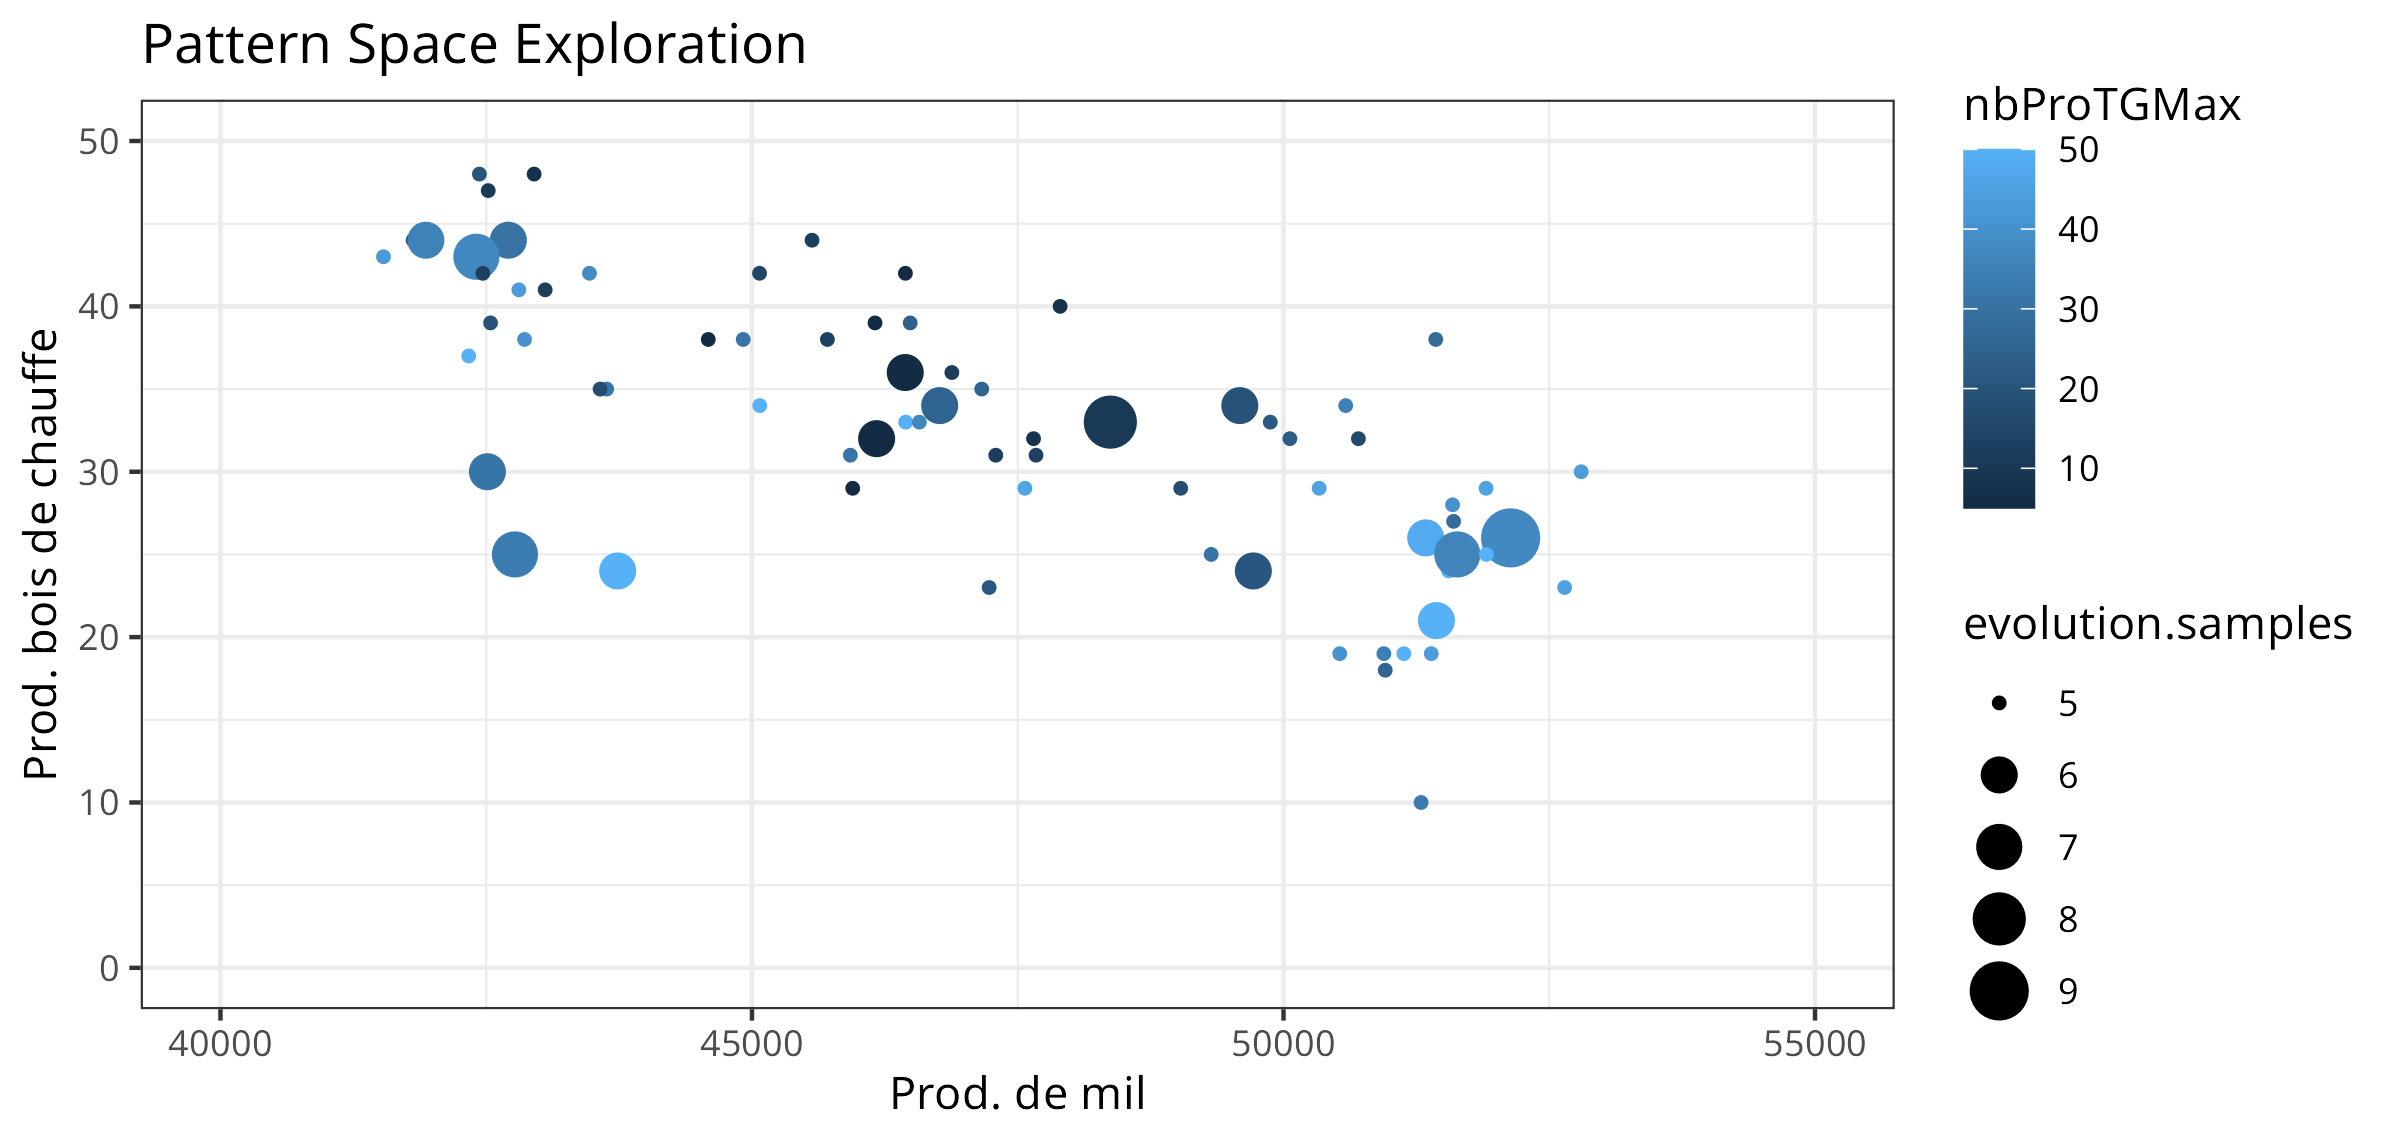
\includegraphics[width=\textwidth]{./img/om_pse.png}
            \caption{Résultat de 33600 évolutions de l'algorithme PSE. Chaque point est un résultat dans l'espace des sorties. La couleur met en évidence le nombre de jeunes pousses protégé par les agriculteurs, et la taille des points donne une idée de la "facilité" pour le modèle à atteindre cet espace. Plus un point est gros, plus le modèle arrive à l'atteindre.}
            \label{fig:PSE}
        \end{figure}

Viabilité du système 

 \subsection{Unexpected Yet Attainable: Surprising Results with Minimal Calculations}

 Dans le cadre de la co-construction du modèle de simulation, en ayant intégré quelques indicateurs de base, nous avons mis en lumière un problème fondamental qui n'avait jusqu'alors jamais été évoqué par les participants du Living-Lab. En suivant attentivement le suivi du nombre d'arbres coupés, que ce soit par les bergers pour le bétail, par les femmes pour le bois de chauffage, ou encore par les agriculteurs lors de leurs activités agricoles, une tendance surprenante est apparue, comme illustré dans la Figure XX. Il ressort de cette analyse que ce sont les agriculteurs eux-mêmes qui contribuent de manière significative à la destruction d'arbres, bien que leur action soit, dans une certaine mesure, silencieuse. Plus précisément, cette destruction passe souvent inaperçue, car elle se manifeste par le désherbage de très jeunes pousses, effectué par les agriculteurs sans qu'ils en aient pleinement conscience. Cette observation remet en question certaines perceptions antérieures et soulève des questions essentielles quant à la gestion des ressources arborées au sein de la communauté.

% The results should describe the experiments performed and the findings observed. The results section should be divided into subsections to delineate different experimental themes. 
% \begin{itemize}
%     \item All data should be presented in the Results. No data should be presented for the first time in the Discussion. Data (such as from Western blots) should be appropriately quantified.
%     \item Subheadings must be either all complete sentences or all phrases. They should be brief, ideally less than 10 words. Subheadings should not end in a period. Your paper may have as many subheadings as are necessary.
%     \item Figures and tables must be called out in numerical order. For example, the first mention of any panel of Fig. 3 cannot precede the first mention of all panels of Fig. 2. The supplementary figures (for example, fig. S1) and tables (table S1) must also be called out in numerical order. 
% \end{itemize}

\section{Discussion}
Include a Discussion that summarizes (but does not merely repeat) your conclusions and elaborates on their implications. There should be a paragraph outlining the limitations of your results and interpretation, as well as a discussion of the steps that need to be taken for the findings to be applied. Please avoid claims of priority. 

\section*{Acknowledgments}

\subsection*{General} 
We warmly thank the residents of Diohine for their hospitality, with special thanks to: Aissatou Faye, Robert Diatte, Pierre Faye, Paul Sene, Ameth Paul Thiaw, Assane Diouf, Guedj Diouf, Nicolas Diouf, Ablaye Faye, Idrissa Faye, Maire-Hélène Ndjira Diouf, Seynabou Gakou, Joseph Sene, Ndeye Thiamal.

\subsection*{Author Contributions} 
Describe contributions of each author to the paper, using the first initial and full last name. 

``L. Broutin conceived the model and realize intervews.''

``E. Delay and L. Broutin animate multi-actor focus groups.''

``E. Delay conducte the HPC exploration.''

``E. Delay and L. Broutin realize the first draft of this manuscript.''

``All authors contributed equally to 2nd version of the manuscript.''

\subsection*{Funding}

This work is part of the research and development project DSCATT (Dynamics of Soil Carbon Sequestration in Tropical and Temperate Agricultural Systems, https://dscatt.net/FR/index.html) co-funded by Agropolis Fondation [reference ID 1802-001] through the "Investissements d'avenir" program Labex Agro [ANR-10-LABX-0001-01] within the framework of I-SITE MUSE [ANR-16-IDEX-0006] and supported by the TOTAL Energies Foundation.

\subsection*{Conflicts of Interest}
The author(s) declare(s) that there is no conflict of interest regarding the publication of this article.

\subsection*{Data Availability}
A data availability statement is compulsory for all research articles. This statement describes whether and how others can access the data supporting the findings of the paper, including 1) what the nature of the data is, 2) where the data can be accessed, and 3) any restrictions on data access and why.

If data are in an archive, include the accession number or a placeholder for it. Also include any materials that must be obtained through a Material Transfer Agreements (MTA). 

\section*{Supplementary Materials}
Describe any supplementary materials submitted with the manuscript (e.g., audio files, video clips or datasets). 

Please group supplementary materials in the following order: materials and methods, figures, tables, and other files (such as movies, data, interactive images, or database files). 

\medskip Example:
Fig. S1. Title of the first supplementary figure.

Fig. S2. Title of the second supplementary figure.

Table S1. Title of the first supplementary table.

Data file S1. Title of the first supplementary data file.

Movie S1. Title of the first supplementary movie.

\medskip
Be sure to submit all supplementary materials with the manuscript and remember to reference the supplementary materials at appropriate points within the manuscript. We recommend citing specific items, rather than referring to the supplementary materials in general, for example: ``See Figures S1-S10 in the Supplementary Material for comprehensive image analysis.''

A link to access the supplementary materials will be provided in the published article.

Supplementary Materials may include additional author notes—for example, a list of group authors.

\section*{Guidelines for References}

There is only one reference list for all sources cited in the main text, figure and table legends, and Supplementary Materials. Do not include a second reference list in the Supplementary Materials section. Include references cited only in the Supplementary Materials at the end of the reference section of the main text; reference numbering should continue as if the Supplementary Materials are a continuation of the main text. References cited only in the Supplementary Materials section are not counted toward length guidelines.

Authors are responsible for ensuring that the information in each reference is complete and accurate.

DOIs, if available, should be included for each reference.

Please do not include any extraneous language such as explanatory notes as part of a reference to a given source. The Journal of Remote Sensing prefers that manuscripts do not include end notes; if information is important enough to include, please put into main text.  If you need to include notes, please explain why they are needed in your cover letter to the editor.

\printbibliography

\end{document}
